\pdfminorversion=7
\PassOptionsToPackage{hyphens}{url}
\documentclass[11pt]{article}
\usepackage[T1]{fontenc}
\usepackage[utf8]{inputenc}
\usepackage{lmodern}
\usepackage[margin=1in]{geometry}
\usepackage{amsmath,amssymb,amsthm,mathtools}
\usepackage{microtype}
\usepackage{enumitem}
\usepackage{tikz}
\usetikzlibrary{arrows.meta,positioning,calc}
\usepackage[hidelinks]{hyperref}
\usepackage{bookmark}
\newcommand{\F}{\mathbb F_2}
\newcommand{\WLdim}{\operatorname{WLdim}}
\newtheorem{theorem}{Theorem}[section]
\newtheorem{lemma}[theorem]{Lemma}
\newtheorem{proposition}[theorem]{Proposition}
\newtheorem{corollary}[theorem]{Corollary}
\theoremstyle{definition}
\newtheorem{definition}[theorem]{Definition}
\theoremstyle{remark}
\newtheorem{remark}[theorem]{Remark}
\numberwithin{equation}{section}
\setlist{itemsep=3pt,topsep=5pt}
\setlength{\emergencystretch}{2em}
\title{The complexity of identifying a graph\newline by Weisfeiler--Leman refinement}
\author{OpenAI}
\date{September 25, 2026}
\hypersetup{pdftitle={The complexity of identifying a graph by Weisfeiler-Leman refinement},pdfauthor={OpenAI}}
\begin{document}
\maketitle
\begin{abstract}
We prove that deciding whether Weisfeiler--Leman refinement of an input
dimension identifies a given graph is EXPTIME-complete. The input is a
nonempty finite simple uncolored graph in adjacency-matrix form and a
positive binary-encoded dimension. Identification quantifies over every
comparison graph.
\end{abstract}
\setcounter{tocdepth}{1}
\tableofcontents
\clearpage
\section{Introduction}
\label{sec:introduction}

The Weisfeiler--Leman algorithm refines the colors of tuples of vertices
to test graph isomorphism. A graph's Weisfeiler--Leman dimension measures how much tuple
information is needed to identify a particular graph among all graphs.
This differs from testing whether a specified pair of graphs survives
refinement: identification quantifies over every possible comparison
graph. We determine the complexity of identification when the dimension
is part of the input.

Increasing the dimension exposes more information, but also increases
the number of tuples on which refinement operates. This makes the least
sufficient dimension a natural measure of the strength needed on an
individual graph. The decision problem studied here asks for that
threshold, rather than for the number of refinement rounds or the cost
of one particular implementation of refinement.

All graphs in this paper are finite, simple, undirected, and uncolored.
For $k\ge2$ we use the joint-update convention: a $k$-tuple starts with
its equality and adjacency type, and each refinement adjoins the
multiset, over vertices $z$, of the vectors of colors obtained by
replacing each coordinate by that same $z$. At $k=1$ we use ordinary
neighbor color refinement. Colors are shared between the graphs being
compared. Write $G\equiv_k H$ when their tuple-color histograms agree
at every round. We say that $k$-WL \emph{identifies} $G$ if
$G\equiv_k H$ implies $G\cong H$ for every graph $H$.
The \emph{Weisfeiler--Leman dimension} $\WLdim(G)$ is the least positive
integer $k$ that identifies $G$. Section~\ref{sec:wl} gives the formal
refinement rule and proves the monotonicity needed for this definition.

Our decision problem has as input a nonempty graph $G$, given by its
binary adjacency matrix, and a positive integer $k$, given in binary.
It asks whether $\WLdim(G)\le k$. Malformed inputs are rejected.

\begin{theorem}
\label{thm:main}
The following problem is EXPTIME-complete under deterministic
polynomial-time many-one reductions: given a nonempty finite simple
undirected uncolored graph $G$ by its adjacency matrix and a positive
integer $k$ in binary, decide whether $\WLdim(G)\le k$.
Here dimension one uses ordinary neighbor color refinement, and
dimensions at least two use the joint-update rule described above.
\end{theorem}

The problem remains EXPTIME-complete when $k$ is encoded in unary
(Corollary~\ref{cor:unary}). Thus the hardness does not require a
dimension whose numerical value is exponentially larger than its encoding.

\subsection{Context and contribution}

The refinement method originates in Weisfeiler and Leman's work on
graph canonization and its associated algebra~\cite{WL1968}.
The relation between Weisfeiler--Leman refinement, counting logic, and
pebble games is a central tool in finite model theory and graph
isomorphism; see Cai, F\"urer, and Immerman~\cite{CFI1992} and the
game formulation in Kiefer and Neuen~\cite{KN2019}.
Arvind, K\"obler, Rattan, and Verbitsky proved P-hardness for
dimension-one identification~\cite{AKRV2017}. Lichter, Ra\ss mann,
and Schweitzer extended fixed-dimension P-hardness to every $k\ge2$
and proved NP-hardness when the dimension is part of the input,
including simple uncolored graphs
\cite[Theorems~3--4]{LRS2025}.
Those results distinguish identification from equivalence of a given
pair. Variable-dimension pair equivalence was shown coNP-hard by
Seppelt~\cite[Theorem~5]{Seppelt2024} and independently by Lichter,
Ra\ss mann, and Schweitzer~\cite[Theorem~19]{LRS2025}.

The identification arguments of Lichter, Ra\ss mann, and Schweitzer
already analyze every equivalent mate of their colored CFI graphs, using
local recognition of gadget incidences
\cite[Lemma~8 and Claim~9]{LRS2024full}. The issue here is therefore
not the all-mates quantifier by itself. Our incidence encoding admits
an entire family of shifted constraints, and we must prove that every
shift arising from an equivalent mate lifts to one global isomorphism
on an accepting instance. This requires more than recognizing the
allowed constraint pattern one incidence piece at a time.

At the level of graph encodings, local parity constraints and a global
twist obstruction are central features of the Cai--F\"urer--Immerman
construction~\cite{CFI1992}. Compressed CFI graphs provide a related
method for retaining game obstructions in smaller representations
\cite{GLNS2025}. That work proves lower bounds on refinement rounds;
such bounds do not by themselves determine the complexity of deciding
identification. Our representation and its game properties are proved
directly below.

The companion paper \emph{Variable-dimension Weisfeiler--Leman
equivalence on general and subcubic graphs}~\cite{VariableWL} develops
a compressed computation construction for pair equivalence. We use its
short tables on binary coordinates, comparisons of images of scalar
linear forms, and potential-based extension of local assignments.
The identification-specific arguments are proved below;
in particular, pair-equivalence hardness is not taken to imply
identification hardness. The graph representation is changed so
that the structure of an arbitrary equivalent graph can be recovered
from bounded-size incidence tests.

Theorem~\ref{thm:main} completes the complexity classification of the
input-dimension identification problem. The additional mechanism is a
local-to-global reconstruction for binary linear constraints. Small
incidence pieces determine the possible shifts in any equivalent graph.
We distinguish local choices that suffice for a winning game strategy
from compatible choices that define one graph isomorphism. Both
conditions are established for an abstract family of comparisons before
the comparisons are chosen to encode a computation.

\subsection{Proof outline}

For a fixed exponential-time machine and input word, the reduction
constructs a graph $G(0)$ and a polynomially bounded dimension $r$.
The graph records binary linear constraints. Each variable bit has a
pair of vertices, and each small constraint has vertices for its legal
valuations, joined to the bit values they specify. Distinct colors for
these classes are subsequently encoded by private leaves. The notation
$G(\beta)$ denotes the same construction with constraint right-hand
sides changed from zero to a list of bits $\beta$.

The representation has three properties. First, every graph equivalent
to $G(0)$ at dimension $r$ is isomorphic to some $G(\beta)$, and such
a mate is isomorphic to $G(0)$ exactly when its shifts admit a global
solution. Second, game equivalence yields nonempty sets of vector
values indexed by binary addresses $a\in\{0,1\}^r$. Each comparison
equates just one scalar image of these sets, up to the prescribed
shift. For a particular class of shifts, these image conditions also
suffice for game equivalence. Third, a global solution exists exactly
when the comparison equations have vector-valued solutions of the form
\[
                  h(a)=\sum_{i=1}^r h_i(a_i,a_{i+1}),
                  \qquad a_{r+1}=a_1,
\]
where each $h_i$ is a function of the displayed two binary coordinates.
The adjacent-coordinate representation is what keeps the graph small
despite its exponentially many addresses.

The addressed comparisons encode a monotone circuit computing the
machine's tableau. A private two-dimensional buffer, compared through
its coordinate forms and their sum, makes a singleton source
image force a singleton destination image, while still permitting
full source images. If the machine accepts, a broadcast family forces
all relevant vector sets to be singletons. Buffered identity
self-connections then compare the same coordinate with both buffer
entries, up to their shifts. Adding the entries cancels the coordinate's
two occurrences and expresses the destination
value as a sum of three shifts. This forces the displayed
adjacent-coordinate form.
Every equivalent mate is therefore isomorphic. If the machine does
not accept, two self-connections admit a shift with no global solution
but with the required nonempty image sets, producing a nonisomorphic
equivalent mate.

Section~\ref{sec:wl} establishes the game convention and the upper
bound. Section~\ref{sec:encoding} gives the incidence construction
and recovers all possible equivalent mates.
Section~\ref{sec:offsets} proves the image conditions and global
lifting criterion. Section~\ref{sec:projection} proves the
local-offset extension theorem underlying the converse game strategy.
Sections~\ref{sec:computation} and~\ref{sec:identification} construct
the computation and complete the reduction, with explicit polynomial
size bounds.

\section{Weisfeiler--Leman refinement and the bijective game}
\label{sec:wl}

We first fix the refinement convention and its game characterization.
The game will let us query the constraints encoded in the graphs of the
next section. It also gives the monotonicity needed to interpret a
dimension bound as identification by a particular refinement algorithm.

All graphs in this paper are finite, simple, undirected, and uncolored
unless colors are explicitly introduced during a construction. For a
graph $G$, an integer $k\ge 2$, and a tuple
$\bar v=(v_1,\ldots,v_k)\in V(G)^k$, let
$\bar v[i\leftarrow z]$ denote the tuple obtained by replacing its
$i$th entry by $z$. The initial color $\chi_0^G(\bar v)$ records every
equality $v_i=v_j$ and adjacency $v_iv_j\in E(G)$. Define subsequent
colors by
\begin{equation}
\label{eq:wl-update}
\chi_{s+1}^G(\bar v)=
\left(\chi_s^G(\bar v),
\left\{\!\left\{
  \bigl(\chi_s^G(\bar v[1\leftarrow z]),\ldots,
        \chi_s^G(\bar v[k\leftarrow z])\bigr)
       :z\in V(G)
\right\}\!\right\}\right).
\end{equation}
Thus a single multiset records the \emph{joint vector} of replacement
colors. It is not a list of separately counted coordinate multisets.
For $k=1$, we instead use ordinary color refinement: all vertices have
one initial color, and
\[
\chi_{s+1}^G(v)=
\left(\chi_s^G(v),
\left\{\!\left\{\chi_s^G(w):w\in N_G(v)\right\}\!\right\}\right).
\]
The colors are named consistently between graphs. Write $G\equiv_k H$
if, at every round, the multisets of colors of their $k$-tuples agree.
We say that $k$-WL \emph{identifies} $G$ if $G\equiv_k H$ implies
$G\cong H$ for every graph $H$. The Weisfeiler--Leman dimension of $G$
is the least positive $k$ that identifies it.

\subsection{The game characterization}

For graphs of equal positive order, the \emph{bijective game with $K$
pair slots} is played as follows. A position consists of at most $K$
pairs of marked vertices, one vertex from each graph in each occupied
slot. Repeated vertices are allowed. Spoiler may discard pairs. To
fill a vacant slot, Spoiler first designates that slot; Duplicator
then announces a bijection $f:V(G)\to V(H)$; finally, Spoiler chooses
$v\in V(G)$ and places the pair $(v,f(v))$ in the designated slot.
Duplicator wins if the occupied pairs always define a partial
isomorphism, preserving equality as well as adjacency. A winning
strategy must work against every sequence of Spoiler's choices.

This is a standard characterization of the joint-vector convention;
see, for example, \cite{KN2019}. We include the argument to fix both
the parameter shift and the treatment of vacant slots.

\begin{lemma}
\label{lem:wl-game}
Let $G,H$ have equal positive order, and let $k\ge 2$. Then
$G\equiv_k H$ if and only if Duplicator has a winning strategy from
the empty position in the bijective game with $k+1$ pair slots.
Moreover, a winning strategy with at least two pair slots implies
$G\equiv_1 H$.
\end{lemma}

\begin{proof}
Apply refinement with common color names to the disjoint union of the
two \emph{tuple tables} $V(G)^k$ and $V(H)^k$, taking replacements
within the corresponding graph. Since each update retains the old
color, these common partitions refine. If one update causes no
splitting, it only renames the existing classes. All subsequent
updates then have the same property, so the common partition has
stabilized.

We use two consequences of the update rule. First, if two tuples have
equal colors at a round, applying the same coordinate permutation to
both preserves color equality. This follows by induction from the
initial types: a common permutation permutes the components of a
replacement vector and applies the corresponding coordinate
permutation to each replacement tuple. Second, for two tuples in the
same stable class, stability provides a vertex bijection matching
their entire vectors of stable replacement colors. Indeed, the two
multisets of such vectors agree, so we may match the vertices within
each vector class.

Suppose $G\equiv_k H$. Choose a pair of equally colored stable
$k$-tuples; one exists because the color histograms agree and the
graphs are nonempty. Use the preceding bijection to append one
vertex to each tuple. The resulting pair of $(k+1)$-tuples has the
following property: deleting any common slot leaves equally colored
stable $k$-tuples. Deleting the appended slot gives the original
pair; every other deletion gives a matched replacement pair, up to
a common coordinate permutation.

Duplicator maintains a pair of fully specified $(k+1)$-tuples with
this property, treating entries in vacant slots as virtual. To fill
slot $j$, apply the stable-class bijection to the projection deleting
slot $j$. Whichever vertex Spoiler chooses, the projection deleting
$j$ remains unchanged, while every other deletion projection becomes
a matched replacement pair, up to a common permutation. Thus the
property persists. Discarding a pair only makes that entry virtual.
Every two slots occur together in some deletion projection because
$k\ge 2$. The initial types in these projections therefore preserve
all equalities and adjacencies among occupied slots, proving that
this strategy wins.

Conversely, fix a winning strategy with $k+1$ slots. We prove by
induction on $s$ that, at every history ending with exactly $k$
occupied pairs, the two tuples have equal round-$s$ colors in any
common ordering of those slots. The case $s=0$ is partial
isomorphism. For the induction step, fill the spare slot. The
strategy announces a bijection before Spoiler chooses the new
vertex. After any such choice, Spoiler may discard any one of the
old slots. The induction hypothesis at these resulting histories
matches all $k$ replacement colors for that same vertex bijection.
Hence the entire joint vector is matched, and
Equation~\eqref{eq:wl-update} gives the next-round equality.

Fill $k$ slots from empty in a fixed order. This procedure induces a
bijection from $V(G)^k$ to $V(H)^k$, even when the strategy depends
on the history. To recover the preimage of a target tuple, invert
the first announced vertex bijection, thereby recover the first
source choice and history, and continue successively. Since each
resulting tuple pair has equal colors at every round, the color
histograms agree.

For the final assertion, use induction on the ordinary
color-refinement round at all one-pair histories. From such a
history fill another slot. The announced bijection preserves
adjacency to the retained pair for every possible choice. After
discarding the old pair, the induction hypothesis matches the
previous-round colors of the new vertices. Thus the same bijection
matches the neighbor-color multisets of the retained vertices.
Their next colors agree. The first announced bijection, from the
empty history, then proves equality of all vertex-color histograms.
\end{proof}

\begin{lemma}
\label{lem:monotonicity}
For positive integers $j\le k$, the relation $G\equiv_k H$ implies
$G\equiv_j H$. Consequently, a graph has Weisfeiler--Leman dimension
at most $k$ if and only if $k$-WL identifies it.
\end{lemma}

\begin{proof}
Equal histograms imply equal graph orders, since their total sizes
are $|V(G)|^k$ and $|V(H)|^k$. Empty graphs cause no difficulty, so
assume that this common order is positive. A winning strategy can
be restricted to a smaller number of slots. For $k\ge j\ge 2$,
apply Lemma~\ref{lem:wl-game} in both directions. For $k\ge 2$ and
$j=1$, use its final assertion; the remaining case is immediate.
If some $j\le k$ identifies $G$, then $k$-equivalence to $G$
implies $j$-equivalence and hence isomorphism. The converse follows
from the definition of dimension.
\end{proof}

The next elementary observation lets us recover vertex colors that
will be encoded by degrees.

\begin{lemma}
\label{lem:degree}
In every history following a winning strategy with at least two pair
slots, matched vertices have equal degrees. Every vertex bijection
announced by that strategy therefore preserves degrees for all its
possible choices.
\end{lemma}

\begin{proof}
Retain only a suspect pair $(v,w)$ and fill another slot. To preserve
adjacency for every vertex choice, the announced bijection must map
$N_G(v)$ onto $N_H(w)$, so their cardinalities agree. This applies to
every candidate pair created by any announced bijection, proving
the second assertion as well.
\end{proof}

\subsection{An exponential-time decision procedure}

\begin{proposition}
\label{prop:upper}
For a nonempty graph given by its binary adjacency matrix and a
positive integer $k$ in binary, deciding whether its
Weisfeiler--Leman dimension is at most $k$ belongs to EXPTIME.
\end{proposition}

\begin{proof}
Malformed encodings, including matrices outside the specified graph
domain and nonpositive parameters, can be rejected in polynomial
time. Let $n\ge 1$ be the order of a valid input graph $G$.

First compare the binary parameter with $n$. If $k\ge n$, accept.
For $n\ge 2$, a $k$-tuple listing all vertices, with repetitions if
needed, has an initial equality and adjacency type that determines
an isomorphism to any matching tuple in a graph of order $n$.
Different orders are distinguished by histogram sizes. Order one
is immediate under ordinary color refinement. This comparison is
performed before constructing a tuple table, regardless of how
large the integer encoded by $k$ may be.

It remains to consider $1\le k<n$. Enumerate all labeled simple
graphs $H$ on $n$ vertices, and reject exactly when one satisfies
$G\equiv_k H$ but $G\not\cong H$. This is the desired test by
Lemma~\ref{lem:monotonicity}. There are
$2^{\binom n2}$ candidates, and testing all $n!$ vertex permutations
per candidate suffices for isomorphism.

For equivalence, maintain integer identifiers for the common color
classes of the two tuple tables. There are $2n^k$ entries and at
most $2n^k$ refinement rounds before stabilization. Each signature
contains the old identifier and at most $n$ vectors of length $k$;
sorting and renaming these signatures costs a fixed polynomial in
$n^k,n,k$. Recursive color expressions need not be expanded.
For $k=1$ use the neighbor signatures instead. Agreement of the
histograms through stabilization is sufficient, since later rounds
only rename stable classes. Finally, $n^k\le n^n$, so enumeration,
refinement, and permutation testing together take time exponential
in a polynomial of the explicit input length.
\end{proof}

\section{Encoding comparisons by locally reconstructible graphs}
\label{sec:encoding}

We now encode scalar comparisons between vector values at binary
addresses. A full-address value will be represented by a sum of $r$
entries, each depending on two consecutive address coordinates. The graph
will encode the table entries through local constraints, without listing
the exponentially many values of their sums.

The construction must also control graphs that were not produced by the
encoding. We will prove that every graph equivalent to the homogeneous
graph has the same constraint pieces, with possibly shifted right-hand
sides. An isomorphism will require one assignment to the shared table
entries satisfying all those shifts simultaneously.

\subsection{Comparisons and subdivided wires}

Throughout the construction we work over the field $\F$, fix
$r\ge 32$, and put $K=r+1$. Indices $i\in\{1,\ldots,r\}$ are cyclic, so
$r+1$ in an address-coordinate index means $1$. A finite nonempty
list of \emph{real types} is given. Each real type $P$ has dimension
$d_P\in\{1,2\}$; a value at type $P$ and address
$a\in\{0,1\}^r$ belongs to $\F^{d_P}$.

A \emph{comparison schema} $e$ consists of ordered real endpoints
$P,R$, a nonempty product domain
\[
D_e=\prod_{i=1}^r D_{e,i},
\qquad \varnothing\ne D_{e,i}\subseteq\{0,1\},
\]
coordinate injections $\sigma_{e,i}:D_{e,i}\to\{0,1\}$, and
scalar linear forms
\[
\lambda_{e,0}:\F^{d_P}\to\F,
\qquad
\lambda_{e,1}:\F^{d_R}\to\F.
\]
Write $\sigma_e(a)=(\sigma_{e,i}(a_i))_{i=1}^r$. The schema
represents comparisons between the first form at $(P,a)$ and the
second form at $(R,\sigma_e(a))$ for every $a\in D_e$. Zero
forms, repeated schemas, parallel schemas, and $P=R$ are all
allowed.

Replace each schema $e:P\to R$ by an oriented \emph{wire}
from $P$ to $R$ with $4K$ private internal types, each of dimension
one. Thus a wire has $4K+1$ links, and different wires have no
internal types in common. The real and internal types, joined by
these links, form the \emph{type layout}. For a type $t$, define its
allowed labels at coordinate $i$ by
\[
A_{t,i}=
\begin{cases}
\{0,1\},&t\text{ is real},\\
D_{e,i},&t\text{ is internal to wire }e.
\end{cases}
\]
Its dimension is denoted by $d_t$, extending the notation for real
types.

Write a link as $\ell=tu$, with $t$ first and $u$ second in its
wire's orientation. At coordinate $i$, its allowed label matches
are
\[
M_{\ell,i}=
\begin{cases}
\{(p,p):p\in D_{e,i}\},
 &\ell\text{ is not the last link of }e,\\
\{(p,\sigma_{e,i}(p)):p\in D_{e,i}\},
 &\ell\text{ is the last link of }e.
\end{cases}
\]
Give each endpoint of $\ell$ a scalar form $L_{\ell,t}$ or
$L_{\ell,u}$. At an internal endpoint this is the identity of
$\F$. At the first real endpoint of the wire it is
$\lambda_{e,0}$, and at the last real endpoint it is
$\lambda_{e,1}$. These assignments refer to the respective wire
ends even when both real endpoints are the same type.

\subsection{Readouts and blocks}

Introduce the following names for vector and scalar variables:
\begin{align*}
x_{i,t,p,p'}&\in\F^{d_t}
 &&(p\in A_{t,i},\ p'\in A_{t,i+1}),\\
y_{i,\ell,p,q}&\in\F
 &&((p,q)\in M_{\ell,i}).
\end{align*}
We call these variables \emph{readouts}; each vector readout has its
fixed ordered bit coordinates. It is useful to regard them as edges
between \emph{corners}, where a corner is a triple $(i,t,p)$ with
$p\in A_{t,i}$. The horizontal readout $x_{i,t,p,p'}$ joins
$(i,t,p)$ to $(i+1,t,p')$. The vertical readout
$y_{i,\ell,p,q}$ for $\ell=tu$ joins $(i,t,p)$ to $(i,u,q)$.

A full allowed address $a\in\prod_i A_{t,i}$ selects one horizontal
readout in each row. These edges form a cycle through the corners
$(i,t,a_i)$. Once values have been assigned to the horizontal names,
their sum
\[
                 h_t(a)=\sum_{i=1}^r x_{i,t,a_i,a_{i+1}}
\]
is the value represented at this address. It is determined by the
short tables $x_{i,t,\cdot,\cdot}$, not assigned independently at each
address. For example, the homogeneous comparison $e:P\to R$ is intended
to impose
\[
 \lambda_{e,0}(h_P(a))
     =\lambda_{e,1}(h_R(\sigma_e(a)))
       \qquad(a\in D_e).
\]
We implement this equality by local equations along the subdivided wire.
Their shifted versions will control the corresponding comparison in an
equivalent graph.

There are two kinds of \emph{blocks}. Each horizontal name $x$ has
one \emph{site block}, using just $x$. For each link $\ell=tu$,
row $i$, and matches
$(p,q)\in M_{\ell,i}$ and
$(p',q')\in M_{\ell,i+1}$, there is a \emph{square block} $B$
using the four names
\[
x_t=x_{i,t,p,p'},\qquad x_u=x_{i,u,q,q'},\qquad
y_i=y_{i,\ell,p,q},\qquad
y_{i+1}=y_{i+1,\ell,p',q'}.
\]
Figure~\ref{fig:square} records these shared names. A valuation of
a block assigns a value to each of its names, in that name's vector
or scalar space.

\begin{figure}[htbp]
\centering
\begin{tikzpicture}[x=1cm,y=1cm,every node/.style={font=\small}]
  \coordinate (tl) at (0,2);
  \coordinate (tr) at (5,2);
  \coordinate (bl) at (0,0);
  \coordinate (br) at (5,0);
  \draw (tl) -- node[midway,above] {$x_t$} (tr);
  \draw (bl) -- node[midway,below] {$x_u$} (br);
  \draw (tl) -- node[midway,left] {$y_i$} (bl);
  \draw (tr) -- node[midway,right] {$y_{i+1}$} (br);
  \fill (tl) circle (1.4pt);
  \fill (tr) circle (1.4pt);
  \fill (bl) circle (1.4pt);
  \fill (br) circle (1.4pt);
  \node[above left] at (tl) {$(i,t,p)$};
  \node[above right] at (tr) {$(i+1,t,p')$};
  \node[below left] at (bl) {$(i,u,q)$};
  \node[below right] at (br) {$(i+1,u,q')$};
\end{tikzpicture}
\caption{A square block at link $\ell=tu$ and row $i$.
Horizontal edges carry vector readouts at their types; vertical
edges carry scalar readouts at the matched labels. Its legal
valuations satisfy Equation~\eqref{eq:square}.}
\label{fig:square}
\end{figure}

Choose one bit $\beta_B\in\F$ for each square block. Every
valuation of a site is legal. A valuation of the displayed square
is legal if
\begin{equation}
\label{eq:square}
L_{\ell,t}(x_t)+L_{\ell,u}(x_u)+y_i+y_{i+1}=\beta_B.
\end{equation}
At least one endpoint of every link is internal, so a square uses
$d_t+d_u+2\le 5$ bit coordinates. The two vertical names are
distinct, and both have coefficient one. Consequently this is a
nonzero linear equation with at most sixteen legal valuations,
the same number for either right-hand side. This remains true when
an endpoint form is zero.

The long wires have a separate role in the game analysis. A collection
of at most $K$ blocks uses at most $K$ layout links, because a site uses
none and a square uses just one. It therefore cannot span a whole wire
of $4K+1$ links. Section~\ref{sec:projection} will use this separation
to extend assignments on small block collections.

The full address space has not been enumerated: each name or block uses
only one coordinate or two consecutive coordinates. We next turn these
bounded-size blocks into a graph in which any equivalent mate must retain
their incidence pattern.

\subsection{The uncolored graph}

First build a graph with indicated vertex colors.
\begin{enumerate}[label=\arabic*.]
\item For each bit coordinate of each readout name, make two
\emph{bit-value vertices}, labeled $0$ and $1$. Give this pair a
fresh color. The same pair is used in every block containing that
coordinate.
\item For each block, make one \emph{valuation vertex} for every
legal valuation, all with a fresh color specific to that block.
Connect a valuation vertex to the bit-value vertex specifying its
assigned value in each coordinate used by the block. Add no other
edges.
\end{enumerate}
This graph is bipartite, with valuation vertices on one side and
bit-value vertices on the other. Call these vertices the
\emph{base vertices}, and let their number be $N$. The number is
independent of the chosen bits $\beta_B$, by the preceding count.
Number the fresh colors, in one common order for all choices of
$\beta$, by $1,\ldots,J$.

To erase the colors, attach $j(N+1)$ new private leaves to each base
vertex of color $j$, and then forget the colors. The resulting
uncolored graph is denoted by $G(\beta)$. Here $\beta$ denotes the
list of all square bits, and $G(0)$ is the graph in which all these
bits vanish. The graph is simple and nonempty, and its order is
independent of $\beta$.

\begin{proposition}[Reconstruction of an arbitrary mate]
\label{prop:mate}
For any comparison data just described, with $r\ge 32$, every graph
$H$ satisfying $H\equiv_r G(0)$ is isomorphic to $G(\beta)$ for
some choice of one bit $\beta_B$ per square block.
\end{proposition}

\begin{proof}
The two graphs have the same positive order, and
Lemma~\ref{lem:wl-game} supplies a winning strategy from $G(0)$ to
$H$ with $K=r+1$ pair slots. We first recover the forgotten colors
and the private leaves, and then recover each block.

A base vertex of color $j$ in $G(0)$ has degree in the interval
\[
I_j=[j(N+1),\ j(N+1)+N-1].
\]
These intervals are pairwise disjoint and lie above degree one.
Every other vertex has degree one. By Lemma~\ref{lem:degree}, the
first announced bijection preserves degrees for every possible
vertex choice. It follows that $H$ has precisely the same number
of vertices in each $I_j$, the same number of degree-one vertices,
and no vertices of other degrees. Call its vertices in $I_j$ base
vertices of color $j$.

Any chosen base vertex of $H$ can be reached in the first
placement, by taking its inverse under the announced bijection.
The next announced bijection must preserve both degrees and
adjacency to that vertex. Its number of degree-one neighbors is
therefore exactly $j(N+1)$. Summing these required counts over
all base vertices accounts for the full number of degree-one
vertices in $H$. Since such a vertex has only one neighbor, all
are private leaves on bases; none remain in a separate component.
The degree intervals continue to preserve base colors throughout
every winning play.

There can be no base edge between two color classes whose vertices
are never adjacent in $G(0)$. Indeed, two arbitrary target vertices
can be reached through two successive placements, using the
inverse of each announced bijection. Their preimages have the
prescribed colors, and partial isomorphism preserves the edge
test. This also rules out edges within either side of the original
bipartition and edges to unrelated bit coordinates.

Fix a block. Mark every one of its valuation vertices in $G(0)$
and both bit-value vertices of each coordinate it uses. For a
square there are at most $16+2\cdot 5=26$ such vertices. A site
has at most four valuations and four bit-value vertices, so is
smaller. All these placements fit within $K\ge 33$ slots. Their
images are distinct, preserve their colors, and exhaust the
corresponding classes in $H$, since the class sizes agree. Thus
the entire colored incidence piece for this block is isomorphic
to its intended piece.

Label the two vertices in every bit pair of $H$ by $0$ and $1$,
once for the whole graph. In a local colored isomorphism, each
bit coordinate is either kept or flipped; different coordinates
cannot be exchanged because they have different colors. The
valuation vertices of a site are therefore precisely all
valuations in these labels. For a square, translating the
homogeneous equation by its coordinate flips changes only the
right-hand side, to some bit $\beta_B$. Its valuation vertices
are exactly the legal valuations of
Equation~\eqref{eq:square} with that bit.

No agreement between the flips used in different local
isomorphisms is being assumed. What is shared is the single
labeling already assigned to each target bit pair, so every
block uses the same coordinates for its incidences. Combining
the resulting block descriptions, the exclusion of other base
edges, and the private leaves gives $H\cong G(\beta)$.
\end{proof}

It remains to distinguish those shifts that merely relabel the
graph. A \emph{global offset assignment} gives a vector in
$\F^{d_t}$ to every horizontal name $x_{i,t,p,p'}$ and a scalar
in $\F$ to every vertical name $y_{i,\ell,p,q}$, with the same
value used in all blocks containing that name. Such an assignment
solves the shifted constraints if it satisfies
Equation~\eqref{eq:square} for every square; sites impose no
additional condition.

\begin{proposition}[Isomorphisms and global offsets]
\label{prop:isomorphism}
For every choice of square bits $\beta$, the graphs $G(0)$ and
$G(\beta)$ are isomorphic if and only if there is a global offset
assignment solving all shifted square constraints.
\end{proposition}

\begin{proof}
An isomorphism preserves degrees, hence every named base-color
class. Its action on each bit pair is a fixed flip. Assemble
these flips into an offset vector for each horizontal name and
an offset scalar for each vertical name. Each block of $G(0)$
has its all-zero valuation vertex. Its image is adjacent to
the bit-value vertices specified by these same offsets, so
its valuation is exactly their restriction to that block.
Legality of the image yields Equation~\eqref{eq:square} with
right-hand side $\beta_B$. Because a bit pair is shared by all
blocks using it, the resulting offsets form one global assignment.

Conversely, suppose such an assignment exists. Translate each
bit pair by its offset, and translate each block valuation by
the offsets on that block's coordinates. Linearity and
Equation~\eqref{eq:square} make the latter a bijection from the
homogeneous legal valuation set to the shifted legal set.
Shared offsets preserve all valuation--bit incidences and
nonincidences. The resulting color-preserving base-graph
isomorphism extends to the private leaves, whose numbers
depend only on the preserved base color.
\end{proof}

Proposition~\ref{prop:mate} reduces the analysis of every
equivalent graph to a list of shifted equations, while
Proposition~\ref{prop:isomorphism} identifies precisely which
lists admit an isomorphism. The next step is to extract
constraints on these shifts from the bijective game and to
express global solvability in terms of full addresses.

\section{Wire comparisons and global offsets}
\label{sec:offsets}

We now relate the small constraints in $G(\beta)$ to values at complete
binary addresses. A winning game gives sets of possible values, with
one scalar image equality for each comparison. A graph isomorphism
requires more: values must be chosen simultaneously and represented
by sums of functions of adjacent coordinates. This section proves
both statements for arbitrary right-hand sides $\beta$.

\subsection{Wire shifts and image sets}

Fix a comparison $e:P\to R$ and $a\in D_e$. Along its wire, use
the address $a$ at the first endpoint and every internal type, and
$\sigma_e(a)$ at the last endpoint. For a link $\ell$ of this wire,
write $B(i,\ell,a)$ for the square specified by these addresses at
row $i$. Define
\begin{equation}
 \Delta_\ell(a)=\sum_{i=1}^r\beta_{B(i,\ell,a)},
 \qquad
 \Delta_e(a)=\sum_{\ell\text{ on }e}\Delta_\ell(a).
 \label{eq:wire-shift}
\end{equation}
All sums in this section are over $\F$. Each summand belonging to
row $i$ depends only on $(a_i,a_{i+1})$.

\begin{proposition}[Image consistency]
\label{prop:image-consistency}
For the construction of Section~\ref{sec:encoding}, suppose
$G(0)\equiv_r G(\beta)$. There are nonempty sets
$Q_{P,a}\subseteq\F^{d_P}$ for every real type $P$ and every
$a\in\{0,1\}^r$ such that, for every comparison $e:P\to R$,
\begin{equation}
 \lambda_{e,0}(Q_{P,a})
   =\Delta_e(a)+\lambda_{e,1}(Q_{R,\sigma_e(a)})
 \qquad(a\in D_e).
 \label{eq:image-consistency}
\end{equation}
Here the equality concerns scalar image sets for one comparison at
a time, not a simultaneous choice of vectors for all comparisons.
\end{proposition}

The condition has a local-support interpretation, as in classical arc
consistency~\cite[Section~4]{Mackworth1977}: each value at either endpoint
has some supporting value at the other endpoint for the one displayed
comparison. Those supports may differ between comparisons. In
particular, even a self-comparison does not require its two endpoint
values to be the same vector. The proposition and its later converse
are proved here for the stated scalar-image condition.

\begin{proof}
Fix a winning $(r+1)$-pair strategy, supplied by
Lemma~\ref{lem:wl-game}. We will define $Q$ using histories in which
Spoiler selects only zero-valuation vertices of blocks in $G(0)$.
Their responses are valuations of the same blocks in $G(\beta)$:
Lemma~\ref{lem:degree} and the degree intervals preserve every base
color.

We first record a consequence of winning that holds at every such
history. If two marked blocks share a readout, their responses agree
on that readout. Otherwise some shared bit has different values.
Discard all pairs except those two and select the zero vertex of
the shared bit pair. It is adjacent to both source blocks, whereas
no vertex of the corresponding target bit pair is adjacent to both
inconsistent target valuations. This contradicts winning. The test
is a hypothetical continuation: it establishes consistency of the
current responses without being performed in the histories used
below. It needs only three pairs after the discards.

For a type $t$ and a full allowed address $a$ at that type, its
\emph{site ring} consists of the $r$ site blocks with readouts
$x_{i,t,a_i,a_{i+1}}$. When their zero valuations are marked, let
$h_t$ be the sum of the response vectors on these readouts.
Starting with this ring and one spare pair, we can transfer the sum
across any incident link with matching addresses.

For each row, place its square's zero valuation before discarding
the old site pair. This uses at most $r+1$ slots, and consistency
copies the horizontal readout at the departure type. After all rows
are replaced, adjacent square responses agree on their shared
vertical readout. Summing Equation~\eqref{eq:square} around this
square ring cancels every vertical value twice. Thus, for the two
horizontal sums $h_t,h_u$ on a link $\ell=tu$,
\begin{equation}
                  L_{\ell,t}h_t+L_{\ell,u}h_u
                  =\Delta_\ell(a).
 \label{eq:link-sum}
\end{equation}
Now replace each square by its arrival-side site, again placing
before discarding. The arrival sum is copied exactly. The procedure
works in either direction. Along a complete wire, the internal
sums are scalars and cancel between consecutive links. We obtain
the endpoint equality with shift $\Delta_e(a)$.

Define $Q_{P,a}$ to be the set of sums obtained from all
zero-block-only histories ending with exactly the site ring at
$(P,a)$ marked. These sets are nonempty because the ring can be
queried from the empty position. They include histories with every
slot ordering. If desired, an ordering can be changed using the
spare slot: duplicate a marked zero-site vertex before discarding
its former pair. Equality forces the duplicate response to agree,
so successive relocations do not change the ring values.

Continue any history realizing a value in $Q_{P,a}$ along the wire
to obtain one image inclusion in
Equation~\eqref{eq:image-consistency}. Starting from any history
realizing a value in $Q_{R,\sigma_e(a)}$ and traversing backward
gives the reverse inclusion. In the backward traversal the
coordinate injections are inverted only on their images. All
resulting histories still consist of zero-block choices.
No memorylessness or common simultaneous vector choice has been
used. This remains true for a loop: returning to the same ring
may produce a different member of its set.
\end{proof}

\subsection{Lifting sums around a cycle}

The preceding proposition imposes only image conditions. To obtain
an isomorphism, we need actual offsets on every shared readout.
The relevant restriction on full-address values is elementary.

\begin{definition}
For a nonempty product $A=\prod_{i=1}^r A_i$ and a vector space $V$
over $\F$, a function $h:A\to V$ has \emph{row-sum form} if there
are functions $h_i:A_i\times A_{i+1}\to V$ such that
\begin{equation}
                 h(a)=\sum_{i=1}^r h_i(a_i,a_{i+1}).
 \label{eq:row-sum}
\end{equation}
Indices are cyclic, so $A_{r+1}=A_1$ and $a_{r+1}=a_1$.
\end{definition}

Restriction to a product subdomain preserves row-sum form, as do
linear maps on $V$ and pullback by coordinatewise maps of the
domain. In particular, all functions in
Equation~\eqref{eq:wire-shift} have row-sum form.

\begin{lemma}[Cycle lifting]
\label{lem:cycle-lifting}
Let $r\ge3$, let each $A_i$ be nonempty, and let
$g_i:A_i\times A_{i+1}\to\F$. If
\begin{equation}
                \sum_{i=1}^r g_i(a_i,a_{i+1})=0
                \qquad\text{for all }a\in\prod_i A_i,
 \label{eq:zero-cycle-sum}
\end{equation}
then there are functions $Y_i:A_i\to\F$ with
$g_i(u,v)=Y_i(u)+Y_{i+1}(v)$ for every $i,u,v$.
\end{lemma}

\begin{proof}
Fix a base address $b$. Taking the rectangular difference in
coordinates $i$ and $i+1$ of Equation~\eqref{eq:zero-cycle-sum}
eliminates all terms except $g_i$, because $r\ge3$. Consequently,
with
\begin{align*}
 c_i&=g_i(b_i,b_{i+1}),\\
 \alpha_i(u)&=g_i(u,b_{i+1})+c_i,\\
 \gamma_i(v)&=g_i(b_i,v)+c_i,
\end{align*}
we have $g_i(u,v)=c_i+\alpha_i(u)+\gamma_i(v)$.
Varying coordinate $i$ alone from the base address gives
$\alpha_i(u)=\gamma_{i-1}(u)$. Evaluation at $b$ gives
$\sum_i c_i=0$.

Choose constants $C_i\in\F$ with $C_i+C_{i+1}=c_i$ cyclically:
choose $C_1$ arbitrarily and recurse, the final equation holding
precisely because the $c_i$ sum to zero. Set
$Y_i(u)=\alpha_i(u)+C_i$. Then
\[
 Y_i(u)+Y_{i+1}(v)
   =c_i+\alpha_i(u)+\gamma_i(v)=g_i(u,v).
\]
For a singleton factor the corresponding deviations vanish, so
the same argument includes that case.
\end{proof}

\subsection{The isomorphism criterion at full addresses}

The image sets extracted from the game may be large, and their scalar
equalities do not choose compatible vectors. We now characterize the
stronger condition needed for an isomorphism: one row-sum function for
each real type, satisfying every comparison pointwise. This criterion
applies to arbitrary square shifts, not only the special twists used
later to construct a counterexample to identification.

\begin{proposition}[Global offsets]
\label{prop:global-offsets}
For any right-hand sides $\beta$ in the construction of
Section~\ref{sec:encoding}, all square equations admit a simultaneous
assignment to the readout names if and only if there are row-sum
functions
$h_P:\{0,1\}^r\to\F^{d_P}$, one for each real type, satisfying
\begin{equation}
 \lambda_{e,0}(h_P(a))+\lambda_{e,1}(h_R(\sigma_e(a)))
       =\Delta_e(a)
 \qquad(e:P\to R,\ a\in D_e).
 \label{eq:global-offsets}
\end{equation}
Equivalently, these functions exist exactly when
$G(0)\cong G(\beta)$.
\end{proposition}

\begin{proof}
Given global offsets, sum their horizontal readouts around every
real-type site ring to define $h_P$. These functions have row-sum
form by definition. Summing the square equations around a link
gives Equation~\eqref{eq:link-sum}, now for the assigned offsets
rather than game responses. Summing along the wire cancels the
internal scalar sums and gives
Equation~\eqref{eq:global-offsets}.

Conversely, suppose the displayed functions exist. At each internal
type $s$ of a wire $e:P\to R$, define a scalar function on $D_e$ by
\begin{equation}
 h_s(a)=\lambda_{e,0}(h_P(a))
       +\sum_{\ell\text{ from }P\text{ through }s}\Delta_\ell(a),
 \label{eq:internal-offset}
\end{equation}
where the sum includes the link arriving at $s$. Every $h_s$ has
row-sum form. Along the first and internal links, the link identity
\eqref{eq:link-sum} follows immediately by cancellation. It holds
also on the last link by Equation~\eqref{eq:global-offsets}, with
$h_R$ evaluated at $\sigma_e(a)$. The latter function remains of
row-sum form in $a$ because the transmission acts coordinatewise.

Choose a row decomposition of each real-type function on the full
binary product, and of each internal-type function on its allowed
product. Assign the chosen row terms to all horizontal readout
names of that type. Each choice is made once per type, so readouts
shared between different incident wires already have consistent
values.

Fix a link $\ell=tu$ on wire $e$. For its matched addresses, denote
the two chosen row-$i$ horizontal values by $x_t$ and $x_u$.
The residual
\[
 g_i(a_i,a_{i+1})=
 \beta_{B(i,\ell,a)}+L_{\ell,t}(x_t)+L_{\ell,u}(x_u)
\]
is a function of those two source coordinates, and the link
identity proves $\sum_i g_i(a_i,a_{i+1})=0$ on $D_e$.
Lemma~\ref{lem:cycle-lifting} supplies functions
$Y_i:D_{e,i}\to\F$ whose consecutive sums equal $g_i$.
Assign $Y_i(a_i)$ to the vertical readout of this link indexed by
the match corresponding to $a_i$.

This assignment is well defined: on every link, including the
last, its matches are indexed bijectively by source-domain labels.
Every square uses an adjacent pair of such labels that extends
to a full address because all other product factors are nonempty.
Thus every square equation is satisfied, not just equations from
a selected collection of addresses. Different links have distinct
vertical readout names, so their assignments are independent.
Site blocks impose no additional constraint. We have obtained
the desired global offsets.

The final equivalence with graph isomorphism is
Proposition~\ref{prop:isomorphism}.
\end{proof}

For later use, note that a row-sum function defined on a product
subdomain of $\{0,1\}^r$ extends to a row-sum function on the whole
cube: extend each of its row terms arbitrarily to the corresponding
binary pair domain. This assertion concerns existence of the
extension, not uniqueness of a row decomposition.

\section{Exact projection and a local game strategy}
\label{sec:projection}

Image consistency is necessary for equivalence by
Proposition~\ref{prop:image-consistency}. We now prove a converse for
twists concentrated in one row and at one end of each wire. This converse
requires only the individual image-set equalities: no simultaneous choice
of values from the sets is assumed.

Choose constants $b_e\in\F$, one for each comparison schema. For a link
$\ell$ on wire $e$, let $b_\ell=b_e$ if $\ell$ is the last link of the
wire and let $b_\ell=0$ otherwise. Set $\delta_r=1$ and $\delta_i=0$
for $1\leq i<r$. Define the square twist by
\begin{equation}
  \beta_B=\delta_i b_\ell
  \qquad\text{when $B$ is a square in row $i$ on link $\ell$.}
  \label{eq:special-twist}
\end{equation}
For this twist, the full-wire sum is $\Delta_e(a)=b_e$ at every
$a\in D_e$.

\begin{theorem}[Special-twist sufficiency]
\label{thm:special-twist}
Consider the graph construction with $r\geq32$ and $K=r+1$.
Let $\beta$ be given by Equation~\eqref{eq:special-twist}. Suppose that,
for every real type $P$ and every $a\in\{0,1\}^r$, there is a nonempty
set $Q_{P,a}\subseteq\F^{d_P}$, and that these sets satisfy
\begin{equation}
  \lambda_{e,0}(Q_{P,a})
  =b_e+\lambda_{e,1}(Q_{R,\sigma_e(a)})
  \qquad(e:P\longrightarrow R,\ a\in D_e).
  \label{eq:special-images}
\end{equation}
Then $G(0)\equiv_r G(\beta)$.
\end{theorem}

Throughout this section assume the hypotheses of the theorem. For each
internal type $s$ of wire $e:P\to R$, define
\begin{equation}
  Q_{s,a}:=\lambda_{e,0}(Q_{P,a})
       =b_e+\lambda_{e,1}(Q_{R,\sigma_e(a)})
       \qquad(a\in D_e).
  \label{eq:internal-image-set}
\end{equation}
These are nonempty scalar sets, independent of the internal type chosen
on that wire. We will assign offsets to the readouts of any collection
of at most $K$ blocks. Each assignment must translate legal homogeneous
valuations to legal shifted valuations. More strongly, every permitted
assignment on a smaller collection must extend to a permitted assignment
on a larger one. This extension property will let Duplicator preserve
old responses while preparing for every possible next vertex.

The sum around one address ring explains the form of these assignments.
Fix a type $t$ and an allowed address $a$, and put a vector $M_i$ at its
corner $(i,t,a_i)$, with $M_{r+1}=M_1$. If the horizontal offset in row $i$ is
$M_i+M_{i+1}+\delta_i h$, with $M_i,h\in\F^{d_t}$, then its sum around
the ring is $h$: every corner vector appears twice, while only row $r$
contributes $h$. We will call the corner vectors \emph{potentials}.
They allow the individual readouts to change while this sum stays fixed.
The proof will determine when the readouts constrain such a sum, and
when a change in the sum can be absorbed into the potentials.

\subsection{Small supports and wrapping addresses}

For a set $U$ of blocks, let $\Gamma_U$ be the undirected graph whose
edges are the readout names appearing in $U$, with their previously
defined corners as endpoints. Repeated names contribute only one edge.
A site contributes one horizontal edge; a square contributes its four
boundary edges. In particular, each block belongs to one connected
component of $\Gamma_U$. The \emph{type support} of a component is the
subgraph of the type layout consisting of its types and links.

\begin{lemma}
\label{lem:small-type-support}
If $|U|\leq K$, every component of $\Gamma_U$ has a type support that
is a tree with at most one real type. A support containing no real type
lies in a single wire interior. A support containing a real type consists
of that type and short arms in its incident wires.
\end{lemma}

\begin{proof}
The support is connected, because it is the image of a connected corner
graph. Each square contributes at most one distinct layout link, while
sites contribute none, so the support has at most $K$ links. Internal
types are private to their wires and have layout degree two. Consequently
a cycle, or a path between distinct real types, must traverse a complete
wire of $4K+1$ links. Neither fits into the support. The remaining
description follows by removing its possible real type.

The same argument allows loops and parallel comparison schemas. In
particular, two arms of one loop-wire may meet at its real endpoint, but
cannot meet again inside that wire without completing its long cycle.
\end{proof}

To compare labels at different types in such a support, fix, for every
link and boundary index, an extension of its label-matching injection to
a permutation of $\{0,1\}$. Use the identity for identity matches and
the inverse permutation when traversing a link backwards. Such
extensions exist because the coordinate maps are injections between
nonempty subsets of a two-element set. Choose a reference type in each
support tree. Transport along its unique paths then expresses all labels
at a given boundary index as labels at the reference type; call these
the \emph{aligned labels}. Every actual vertical edge preserves its
aligned label. On a connected subtree, the inherited alignment and the
alignment at a new reference differ only by re-expression at that
reference. This construction does not assert that every ambient label is
allowed at every internal type.

Give each horizontal edge in row $i$ the marker $\delta_i$, and each
vertical edge marker zero. A block collection, or a component of its
corner graph, is \emph{wrapping} if its corner graph has a closed walk
whose marker sum in $\F$ is one. Thus wrapping means that some closed
walk crosses the row-$r$ seam an odd number of times. Traversals in either
direction have the same marker.

\begin{lemma}[Wrapping addresses]
\label{lem:wrapping-address}
Let $|U|\leq r+1$.
\begin{enumerate}
\item Every wrapping subcollection of $U$ has at least $r$ blocks.
\item A wrapping collection of exactly $r$ blocks has one block in
each row, lies in one component, and determines a full address in that
component's aligned labels.
\item All wrapping $r$-subcollections of $U$, if any, lie in one
component of $\Gamma_U$ and determine the same aligned address there.
\end{enumerate}
\end{lemma}

\begin{proof}
For a closed walk, let $c_i\in\F$ be its horizontal traversal count
in row $i$, reduced modulo two. Summing incidences at all corners with
boundary index $i$ gives $c_{i-1}=c_i$: vertical traversals contribute
twice. An odd marker means $c_r=1$, so every row has an odd horizontal
traversal count. Since a block supplies horizontal edges in only its own
row, at least $r$ blocks are needed.

If there are exactly $r$ blocks, there is one in each row, and the walk
meets every block. Thus all blocks lie in its component. The horizontal
edge of a site, or the two horizontal edges of a square, prescribes one
pair of aligned labels for that row. In the square case the two edges
give the same pair because vertical edges preserve alignment. Now sum
the walk's incidences separately at each aligned label of boundary
index $i$. Vertical contributions again cancel. The odd horizontal
traversal counts in the adjacent rows force their prescribed labels at
this boundary to agree. Doing this at every boundary gives the full
address.

Two $r$-subcollections of $U$ share at least $r-1$ blocks. For wrapping
subcollections these common blocks belong to distinct rows and put both
subcollections in the same component. The common rows, all but at most
one row, touch every boundary index because $r\geq3$. Hence they force
the two addresses to agree at every coordinate.
\end{proof}

\subsection{Translations on a small block collection}

We next define the translations that will be available to Duplicator.
The address condition will be imposed only when a wrapping collection
of exactly $r$ blocks is present. A wrapping component with $r+1$
blocks need not contain such a collection; this distinction is essential
when restricting to smaller collections.

Fix $U$ with $|U|\leq K$. In each component $C$ of $\Gamma_U$, choose
a vector $h_t\in\F^{d_t}$ for each type in its support, subject to
\begin{equation}
  L_{\ell,t}(h_t)+L_{\ell,u}(h_u)=b_\ell
  \qquad(\ell=tu\text{ in the support}).
  \label{eq:component-shifts}
\end{equation}
The choices are made separately in distinct corner components, even
when the same type occurs in more than one component. If $C$ contains
a wrapping $r$-subcollection, use its unique aligned address from
Lemma~\ref{lem:wrapping-address} and impose one further condition:
\begin{itemize}
\item If the support contains a real type $P$, require
$h_P\in Q_{P,a}$, where $a$ is the address expressed at $P$.
\item If the support has no real type, require its common internal
scalar to lie in $Q_{s,a}$, where $a$ is expressed in the source
coordinates of its wire.
\end{itemize}
In the second case, $a\in D_e$: every boundary label of the wrapping
collection is read at an internal type of wire $e$, and its interior
matches are identities. In the first case every address is permitted
at $P$; there is no additional address-dependent condition on its arms.
If no wrapping $r$-subcollection is present, impose only
Equation~\eqref{eq:component-shifts}. Call shifts satisfying these
requirements \emph{admissible}.

Admissible shifts always exist. In a wire interior all $b_\ell$ vanish,
so one common scalar, in the indicated nonempty set when required,
suffices. If the support contains a real type, choose its vector
arbitrarily or from the indicated nonempty $Q$ set. Its endpoint forms
then determine the scalar on each arm, adding the last-link constant
when that arm meets the second endpoint of a wire. The scalar is
constant along the rest of the arm. Distinct arms have private internal
types, so these choices do not conflict, even when an endpoint form
vanishes.

Independently choose a potential $M_v\in\F^{d_t}$ at every corner $v$
of type $t$. Define offsets on the readouts by
\begin{equation}
\begin{aligned}
  x_{vw}&=M_v+M_w+\delta_i h_t
    &&\text{for a horizontal edge in row $i$ at type $t$},\\
  y_{vw}&=L_{\ell,t}(M_v)+L_{\ell,u}(M_w)
    &&\text{for a vertical edge on $\ell=tu$}.
\end{aligned}
\label{eq:potential-offsets}
\end{equation}
The endpoints of the vertical edge are ordered as in its readout name.
Let $\mathcal H_U$ be the family of all assignments to the readout names
of $U$ obtained this way. Set $\mathcal H_\varnothing=\{\varnothing\}$.
Every family is nonempty. In a square, the potential terms cancel and
the remaining offset sum is
\[
  \delta_i\bigl(L_{\ell,t}(h_t)+L_{\ell,u}(h_u)\bigr)
  =\delta_i b_\ell=\beta_B.
\]
Thus every assignment in $\mathcal H_U$ satisfies
Equation~\eqref{eq:square} on all squares in $U$. It translates every
homogeneous block valuation into a legal valuation for the twist.
Shared readouts receive the same offsets because they are the same
edges of $\Gamma_U$. Figure~\ref{fig:projection-gauge} shows how the
potentials preserve old readouts when a site ring is cut. The next proof
extends this adjustment to every nonwrapping component.

\begin{figure}[htbp]
\centering
\begin{minipage}[t]{0.47\linewidth}
\centering
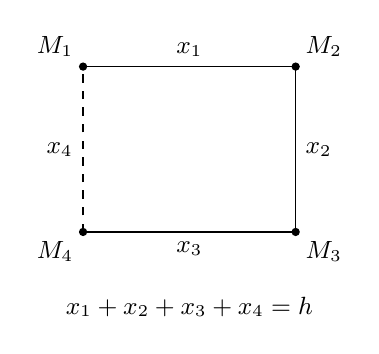
\begin{tikzpicture}[font=\small,line width=0.5pt]
 \coordinate (v1) at (0,0);
 \coordinate (v2) at (2.7,0);
 \coordinate (v3) at (2.7,-2.1);
 \coordinate (v4) at (0,-2.1);
 \draw (v1)--node[above]{$x_1$}(v2)
       --node[right]{$x_2$}(v3)
       --node[below]{$x_3$}(v4);
 \draw[dashed,thick] (v4)--node[left]{$x_4$}(v1);
 \foreach \v in {v1,v2,v3,v4} \fill (\v) circle (1.5pt);
 \node[above left] at (v1) {$M_1$};
 \node[above right] at (v2) {$M_2$};
 \node[below right] at (v3) {$M_3$};
 \node[below left] at (v4) {$M_4$};
 \node at (1.35,-3.05) {$x_1+x_2+x_3+x_4=h$};
\end{tikzpicture}
\end{minipage}\hfill
\begin{minipage}[t]{0.50\linewidth}
\centering
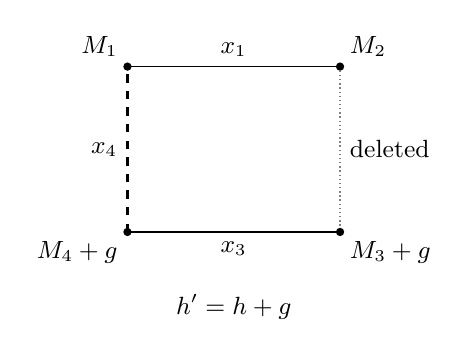
\begin{tikzpicture}[font=\small,line width=0.5pt]
 \coordinate (v1) at (0,0);
 \coordinate (v2) at (2.7,0);
 \coordinate (v3) at (2.7,-2.1);
 \coordinate (v4) at (0,-2.1);
 \draw (v1)--node[above]{$x_1$}(v2);
 \draw[densely dotted,gray] (v2)--node[right,text=black]{deleted}(v3);
 \draw (v3)--node[below]{$x_3$}(v4);
 \draw[dashed,thick] (v4)--node[left]{$x_4$}(v1);
 \foreach \v in {v1,v2,v3,v4} \fill (\v) circle (1.5pt);
 \node[above left] at (v1) {$M_1$};
 \node[above right] at (v2) {$M_2$};
 \node[below right] at (v3) {$M_3+g$};
 \node[below left] at (v4) {$M_4+g$};
 \node[align=center] at (1.35,-3.05)
   {$h'=h+g$};
\end{tikzpicture}
\end{minipage}
\caption{A schematic site ring at one type and one address, drawn with four
rows; the construction itself uses $r\ge32$. Here $x_i$ is the horizontal
offset in row $i$, and $g$ is any vector in the same space as $h$.
The dashed edge is the row-$4$ seam. Left: every potential occurs twice in the sum, leaving $h$.
Right: after deleting row $2$, changing $h$ to $h+g$ and adding $g$ to
$M_3,M_4$ preserves every retained readout. The dotted segment is absent
from the retained corner graph. The proof of
Proposition~\ref{prop:exact-projection} makes this adjustment on each
nonwrapping old component, including components meeting several types. Adapted from \cite[Figure~2]{VariableWL}.}
\label{fig:projection-gauge}
\end{figure}

\subsection{Exact projection}

The families just constructed provide legal translations on small
collections. Their usefulness in the game depends on preserving every
old readout when the block collection grows.

A proper old collection has at most $r$ blocks. If an old component
wraps, it uses all $r$ of them and carries the only old choice subject to
an address-set condition. We will retain its chosen shifts, or lift its
scalar through an endpoint form. On every other old component,
the marker can be expressed as a sum of binary values at the edge
endpoints. There we can change the component shifts and compensate by
changing potentials, leaving all old
readouts unchanged. These are the two cases of the following proof.

\begin{proposition}[Exact projection]
\label{prop:exact-projection}
For $V\subseteq U$ with $|U|\leq r+1$, restriction to the readout names
occurring in $V$ maps $\mathcal H_U$ onto $\mathcal H_V$.
\end{proposition}

\begin{proof}
The assertion is immediate for $V=U$. Assume $V\subsetneq U$, so
$|V|\leq r$. Each component $D$ of $\Gamma_V$ lies in a component
$C$ of $\Gamma_U$, and its type support is a subtree of that of $C$.

\emph{Restriction of admissible shifts.}
If $D$ is nonwrapping,
it has no $Q$ requirement, so restriction causes no problem. If $D$
wraps, its blocks form a wrapping $r$-collection by
Lemma~\ref{lem:wrapping-address}; in particular they exhaust $V$.
The address imposed on $C$ restricts to the same address on $D$.
When $D$ contains a real type, it is the same real type as in $C$ and
has the same $Q$ requirement. When $C$ has no real type, both supports
are in one wire interior and require the same common scalar.

The remaining case is that $D$ lies inside a wire and $C$ reaches one
of its real endpoints. The address $a$ read inside $D$ belongs to the
actual product domain $D_e$. Consequently its expression at the real
endpoint uses actual endpoint matches: it is $a$ at the first endpoint
and $\sigma_e(a)$ at the second. By
Equation~\eqref{eq:internal-image-set}, the permitted internal scalar
set is exactly the image of the permitted real-vector set under the
endpoint form, translated by the end-link constant if present.
Restriction is therefore admissible. The same equality shows that any
permitted internal scalar has a permitted real-vector preimage.

\emph{Extension from a wrapping old component.}
These cases also show that admissible shifts on a wrapping old component
extend to admissible shifts on its containing new component: retain its
real vector if already present, retain its scalar if the new support
remains internal, or choose the real preimage just described. Then
extend along the remaining arms. Only one arm is constrained in the
preimage case. Since a wrapping old component consumes all $r$ old
blocks, there is never a second old wrapping choice to lift
simultaneously. This remains true for loop-wires whose two original
endpoints are the same real type.

\emph{Preservation of every old readout.}
Restricting the potentials as well now proves that every restriction of
an element of $\mathcal H_U$ lies in $\mathcal H_V$. For surjectivity,
fix a representation of an element of $\mathcal H_V$ by old shifts and
potentials. Choose admissible shifts on $U$, agreeing with the old
shifts on the possible wrapping old component; the preceding argument
shows this is possible. We will adjust potentials to preserve the old
readouts on every nonwrapping component $D$.

On such a component, the marker is a difference of corner labels:
there are $s_v\in\F$ with marker $s_v+s_w$ on each edge $vw$.
Indeed, choose path sums from one fixed corner. They are well-defined
because every closed walk has marker sum zero. Let $g_t$ be the sum of
the new and old shifts at type $t$ in this component. Their identical
inhomogeneous link equations imply
\[
  L_{\ell,t}(g_t)+L_{\ell,u}(g_u)=0
  \qquad(\ell=tu\text{ in the support of }D).
\]
Replace the old potential at $v$ of type $t$ by $M_v+s_vg_t$.
For a horizontal edge in row $i$, the resulting change in its offset,
including the change of shift, is
\[
  (s_v+s_w+\delta_i)g_t=0.
\]
For a vertical edge, $s_v=s_w$, and the homogeneous link equation makes
its offset change zero as well. Hence every old readout is preserved.

Different old components have disjoint corners, so their potential
adjustments are compatible even if they merge in $\Gamma_U$ or contain
the same type. Retain the old potentials on a wrapping old component
and choose arbitrary potentials at all new corners. Together these
choices give an element of $\mathcal H_U$ extending the prescribed
element of $\mathcal H_V$.
\end{proof}

In particular, a wrapping $(r+1)$-block component with no wrapping
$r$-subcollection causes no exceptional case. Every proper subcollection
has at most $r$ blocks and is nonwrapping, so the potential adjustment
in the proof applies without a $Q$ restriction.

\subsection{From translations to a vertex bijection}

We can now prove Theorem~\ref{thm:special-twist}. Fix the following
ownership convention, identically in $G(0)$ and $G(\beta)$. A block's
valuation vertices are owned by that block. Each bit-value pair is
owned by one fixed block using its readout name. Such a block exists:
horizontal names have sites, and every vertical name belongs to a
square because the adjacent coordinate domains are nonempty. A leaf
has its parent's owner and a fixed private index among the leaves at
that parent.

\begin{proof}[Proof of Theorem~\ref{thm:special-twist}]
Duplicator maintains an assignment in $\mathcal H_U$, where $U$ is
the set of owners of the currently marked vertices. Marked base
vertices are matched by translation using the offsets on their
owners: translate each block valuation and each bit-value coordinate.
A marked leaf is sent to the leaf with the same private index at the
translated parent. Since $|U|$ is at most the number of occupied slots,
the family $\mathcal H_U$ is always defined.

For any fixed assignment, translation is bijective on every base
vertex class with owner in $U$: it maps homogeneous legal valuations
onto the legal valuations for the twist, and permutes each bit-value
pair. Parent translation also gives a bijection on the corresponding
leaves, since translated parents have the same color and hence the
same number of attached leaves.

These translations give a partial isomorphism on the marked vertices.
The only possible base incidence is between a block valuation and a
bit-value vertex for a coordinate used by that block. When both are
marked, their owners belong to $U$ and the common readout receives
one offset. Equality or inequality of the two bits is therefore
preserved, so both adjacency and nonadjacency are preserved. All other
pairs of base classes have no edges in either graph. Leaf attachments
are preserved by parent translation and private indices. Translation
within each class is injective, distinct classes remain distinct, and
leaf indices are preserved, so equality of marked vertices is
preserved as well.

Discarding pairs simply restricts the maintained assignment to the
remaining owners, which is allowed by
Proposition~\ref{prop:exact-projection}. Suppose now that a slot is
vacant. There are at most $K-1=r$ current owners. For \emph{each}
possible owner $B$ of the next vertex, choose an extension of the
current assignment to $\mathcal H_{U\cup\{B\}}$. This is possible
before any vertex is selected, by exact projection. If $B\in U$, use
the current assignment itself.

On the part of the vertex set owned by $B$, use the chosen extension
to translate the base classes and their leaves. These parts partition
the vertex set, and each maps bijectively onto the identically owned
part in the other graph. They therefore combine into a single vertex
bijection, which Duplicator announces. Its parts for the current
owners agree with the maintained assignment, so in particular it
extends all currently marked pairs, including repeated occurrences of
a vertex.

After Spoiler selects a vertex, retain the extension chosen for its
owner $B$. It agrees with every old marked pair and with the newly
selected pair. The preceding partial-isomorphism check applies to
this enlarged position. Thus the strategy wins with $K=r+1$ slots,
which proves $G(0)\equiv_r G(\beta)$.
\end{proof}

\section{A computation described by product schemas}
\label{sec:computation}

We now use a polynomial-size description of an exponentially large
monotone circuit. Its true gates will specify which scalar images must become
singletons in an equivalent graph. We apply the uniform product-circuit
compilation theorem from the companion paper \cite{VariableWL}, with
stronger address padding. The next section
supplies all additional constraints needed for identification.

Fix a binary language in \(\mathrm{EXPTIME}\).  Choose a fixed deterministic
machine \(M\) deciding it, with a single doubly infinite tape. Its input
occupies positions \(0,\ldots,m-1\), all other cells are blank, and its
head starts at zero and moves by at most one cell per step. Its running time is at most
\[
 T=2^{p(m)},
\]
where \(m\) is the input length and \(p\) is a fixed polynomial with integer
coefficients satisfying \(p(m)\ge m+32\).  These conventions cause no loss of
generality.  A fixed multitape machine can be simulated on one tape using
tracks and head markers: sweeps of the used interval find the scanned symbols
and then update the symbols and head positions.  After \(t\) simulated steps,
the interval has length \(O(m+t+1)\), so the overhead is polynomial and can be
absorbed into \(p\).  We also arrange that a halted machine leaves its tape and
head unchanged, retaining its accepting or rejecting state.

For an input word \(w\) of length \(m\), put
\begin{equation}
 d=p(m)+2,\qquad S=2^d=4T,\qquad r=2d.
 \label{eq:computation-parameters}
\end{equation}
In particular $r\ge68$, so the reconstruction and special-twist results
requiring $r\ge32$ apply. Enlarging a valid exponential-time bound to
meet this padding condition changes neither the fixed machine nor its
accepted language.
An address in \(\{0,1\}^r\) consists of two groups of \(d\) bits, in increasing
place order, representing \((\tau,j)\) with \(0\le \tau,j<S\).  Time \(\tau\)
is not cyclic; the position \(j\) is taken modulo \(S\).

We use two kinds of monotone gates.  A scalar gate takes the OR of its incoming
connections and is also true if designated as a seed.  A two-port AND gate
takes the OR of the connections to each port and then the AND of the two port
values.  An empty OR is false.  Each gate type has one gate at every address.
A connection schema specifies its source type, its destination type and port,
a nonempty product source domain, and coordinate injections carrying the
source address to the destination address.  Thus its address data have exactly
the form of a comparison schema from the preceding sections.  A seed or test
request specifies a scalar type and a product of allowed address coordinates.

\begin{proposition}
\label{prop:computation}
For the fixed machine \(M\) and each input \(w\), with parameters
\eqref{eq:computation-parameters}, one can construct in time polynomial in
\(r+m\) an acyclic monotone circuit description with \(O_M(1)\) gate types and
\(O_M((r+1)^2+m)\) connection schemas, seed requests, and test requests.
Every schema has a nonempty product domain and coordinate injections;
the whole description contains \(O_M(r((r+1)^2+m))\) constant-size
coordinate entries. All tests are scalar terminal gates.
The machine \(M\) accepts \(w\) if and only if at least one designated test
gate is true.
\end{proposition}

\begin{proof}
Apply the uniform product-circuit compilation theorem
\cite[Proposition~3.2]{VariableWL} to \(M,p\). It uses the same
one-tape initialization and frozen-halting convention, the same two
least-significant-bit-first coordinate groups, and the same address
length \(r=2(p(m)+2)\). Its position ring has length \(4T=S\),
and its requirement \(p(m)\ge m+2\) is satisfied by our padding.
The theorem gives the stated counts and polynomial-time generation.

The construction uses a fixed local transition rule on three neighboring
tape cells. Scalar gates record cell symbols, and two-port AND gates
recognize the triples producing each next symbol. Time increment and
position increment or decrement are split into carry and borrow cases.
Each case fixes some bits and flips or preserves each coordinate,
so its domain is a product and its coordinate maps are injections.
Combining time and position cases gives \(O_M(r^2)\) connection schemas.
The exceptional input cells and a product decomposition of the blank
suffix supply the seed requests; final-time accepting symbols supply
the terminal tests. The compiler generates these short tables without
listing full addresses. Applied to the decider \(M\) for the chosen
language, its true-test condition is exactly acceptance of \(w\).
\end{proof}

\section{From acceptance to identification}
\label{sec:identification}

Apply Proposition~\ref{prop:computation} to the fixed machine \(M\) and input
\(w\).  We turn its circuit description into comparison schemas, then use the
graph construction of the preceding sections.  The additional comparisons
serve two purposes: an accepting test will force singleton values at every
gate type and at an additional broadcast type, at all addresses, and coordinate
self-connections will make those values row-sum functions.  Both properties
are needed to identify the graph among all its equivalent mates.

\subsection{Real types and buffered connections}

Give each scalar gate type dimension one, with its scalar coordinate as both
input and output form.  Give each AND type dimension two: the input forms are
the coordinate projections and the output form is their sum.  Introduce a
further scalar type \(A\), called the broadcast type.  The gate types and
\(A\) will be called the \emph{primary types}.  Also introduce a scalar dummy
type.  For each seed request, add a comparison from the specified scalar
type to the dummy on that request's product domain, with identity address
transmission, comparing the scalar form at the source with the zero form at
the dummy.  The dummy has no other use.

Regard the circuit connections as directed connections from a source output
form to a destination input form.  Add the following directed connection
schemas:
\begin{enumerate}
\item From each tested scalar type to \(A\), on its test domain and with
identity address transmission.
\item For each address coordinate \(i\), from \(A\) to \(A\) on the full
product, flipping coordinate \(i\) and leaving the others unchanged.
\item From \(A\) to every coordinate form of every gate type, on the full
product with identity address transmission.
\item From every coordinate form of every primary type to itself, on the full
product with identity address transmission.  For the coordinate of \(A\),
include two distinct copies of this self-connection.
\end{enumerate}
These added connections describe constraints; they are not included when
evaluating the acyclic circuit from Section~\ref{sec:computation}.

One-way propagation is a central feature of Grohe's monotone-circuit
reductions for finite-variable equivalence~\cite{Grohe1999} and of the
later identification construction of Lichter, Ra\ss mann, and Schweitzer
\cite[Section~5]{LRS2025}. Here private two-coordinate scalar-image
buffers implement the directional effect. Their exact properties,
including the shifted comparisons needed for arbitrary mates, are
proved below rather than imported from those graph switches.

Implement each directed connection schema \(l\), original or added, using a
private real type \(B_l\) of dimension two.  Suppose \(l\) goes from a form
\(o\) on a primary type \(P\) to a form \(s\) on a primary type \(R\), with
source domain \(D_l\) and address map \(\sigma_l\).  The two coordinate
forms of \(B_l\) are denoted by \(z_1,z_2\), and its addresses use the source
coordinate system.  Add precisely three comparison schemas:
\begin{equation}
\begin{array}{c|c|c|c}
 \text{schema}&\text{source form}&\text{destination form}
       &\text{address map on }D_l\\ \hline
 l1&o\text{ on }P&z_1\text{ on }B_l&\mathrm{id}\\
 l2&o\text{ on }P&z_2\text{ on }B_l&\mathrm{id}\\
 l3&z_1+z_2\text{ on }B_l&s\text{ on }R&\sigma_l
\end{array}
\label{eq:buffer}
\end{equation}
There is no other use of \(B_l\), and all three schemas have source domain
\(D_l\).  In particular, splitting a connection family into several product
schemas gives a separate buffer for each schema.

The reason for comparing the two coordinates separately is already
visible in the set $\{(0,0),(1,1)\}\subseteq\F^2$: each coordinate
image is all of $\F$, although the sum image is $\{0\}$.
Similarly, $\{(0,1),(1,0)\}$ has full coordinate images and sum image
$\{1\}$. Thus the buffer can retain two full source images while
restricting their sum. In the other direction, fixing both coordinate
images to singletons forces the entire nonempty buffer set to be a
singleton. These are the two behaviors used in the acceptance and
nonacceptance arguments below.
Figure~\ref{fig:buffer} separates the three comparison constraints
from the operation of adding the buffer's two coordinates.

\begin{figure}[htbp]
\centering
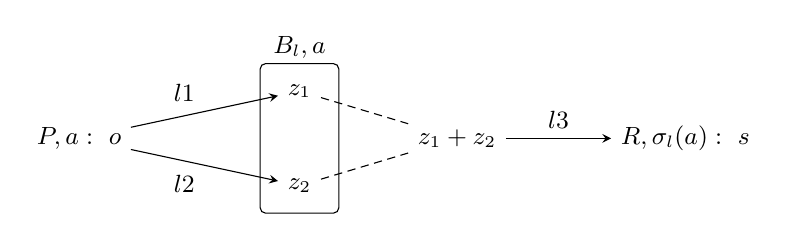
\begin{tikzpicture}[>=stealth, every node/.style={font=\small}]
 \node (source) at (0,0) {\(P,a:\ o\)};
 \node (one) at (2.8,.6) {\(z_1\)};
 \node (two) at (2.8,-.6) {\(z_2\)};
 \node at (2.8,1.15) {\(B_l,a\)};
 \draw[rounded corners=2pt] (2.3,-.95) rectangle (3.3,.95);
 \node (sum) at (4.8,0) {\(z_1+z_2\)};
 \node (target) at (7.7,0) {\(R,\sigma_l(a):\ s\)};
 \draw[->] (source) -- node[above left] {\(l1\)} (one);
 \draw[->] (source) -- node[below left] {\(l2\)} (two);
 \draw[densely dashed] (one) -- (sum);
 \draw[densely dashed] (two) -- (sum);
 \draw[->] (sum) -- node[above] {\(l3\)} (target);
\end{tikzpicture}
\caption{A buffered connection.  Solid arrows represent the three comparisons
in \eqref{eq:buffer}; dashed lines indicate addition of the two coordinates,
not further comparisons.  Image consistency compares sets of form values,
with their shifts.  It does not choose a common pointwise value for all
comparisons.}
\label{fig:buffer}
\end{figure}

Apply the layout and graph construction to exactly the seed comparisons and
the triples \eqref{eq:buffer}, and output
\begin{equation}
 (G(0),r),
 \label{eq:reduction-output}
\end{equation}
with \(r\) as in \eqref{eq:computation-parameters}.  All real-type dimensions
are one or two, all domains are nonempty products, and all address maps are
coordinate injections.  Thus the hypotheses of the graph construction hold.

\subsection{Acceptance: every equivalent mate is isomorphic}

\begin{proposition}
\label{prop:acceptance}
If \(M\) accepts \(w\), then every finite simple uncolored graph
\(H\equiv_r G(0)\) is isomorphic to \(G(0)\).
\end{proposition}

\begin{proof}
By Proposition~\ref{prop:mate}, write \(H\cong G(\beta)\) for some square
bits \(\beta\).  Transporting equivalence through this isomorphism, apply
Proposition~\ref{prop:image-consistency} to obtain nonempty sets
\(Q_{P,a}\) satisfying \eqref{eq:image-consistency}.  No restriction to the
special twists of Theorem~\ref{thm:special-twist} is made here: all wire sums
\(\Delta_e(a)\) may depend on the address.

First consider a buffered connection \(l\) at \(a\in D_l\).  If the source
image \(o(Q_{P,a})\) is a singleton, the first two comparisons force both
coordinate images of \(Q_{B_l,a}\) to be singletons, possibly translated by
different shifts.  As this set is nonempty, it contains exactly one vector.
Its sum image is therefore a singleton, and the third comparison makes
\(s(Q_{R,\sigma_l(a)})\) a singleton.  Thus a buffered connection propagates
singletonness from its source form to its destination form.  We do not need
these singletons to have value zero.

At each seed, comparison with the dummy's zero form gives a singleton scalar
image.  Induction in the acyclic circuit order now shows that every true gate
has a singleton output image.  For a true scalar, use its seed comparison or
one true incoming source.  For a true AND gate, each port receives a true
source, so both coordinate images become singletons and their sum is a
singleton as well.

By Proposition~\ref{prop:computation}, at least one test is true.  Its added
connection forces \(A\) to have a singleton image at that address.  Flipping
individual coordinates connects all addresses in \(\{0,1\}^r\), so the
broadcast connections propagate this property to every address of \(A\).
The connections from \(A\) to every gate coordinate then imply that all
primary sets are singletons.  Write
\[
 Q_{P,a}=\{h_P(a)\}
 \qquad(P\text{ primary},\ a\in\{0,1\}^r).
\]

To use Proposition~\ref{prop:global-offsets}, it remains to prove that these
functions have row-sum form and to supply the functions at the remaining real
types.  Fix a coordinate form \(s\) of a primary type \(P\), and take its
identity self-connection \(l\).  At each address, the first two comparisons
give buffer coordinates
\[
 z_1=s(h_P(a))+\Delta_{l1}(a),\qquad
 z_2=s(h_P(a))+\Delta_{l2}(a).
\]
Their sum cancels the two copies of \(s(h_P(a))\) over \(\F\).  The third
comparison, with destination the same coordinate at the same address, gives
\begin{equation}
 s(h_P(a))=\Delta_{l1}(a)+\Delta_{l2}(a)+\Delta_{l3}(a).
 \label{eq:self-connection-row-sum}
\end{equation}
Each term on the right has row-sum form on the full product.  Hence every
coordinate of every primary \(h_P\) has row-sum form, and therefore so does
the vector function itself.  Either self-connection copy suffices for \(A\).

For each private buffer \(B_l\), prescribe on \(D_l\) its coordinates
\[
 h_{B_l,j}(a)=o(h_P(a))+\Delta_{lj}(a),\qquad j=1,2.
\]
These are the unique coordinates of its image-consistency set on that domain.
They have row-sum form there.  Extend each adjacent-coordinate term arbitrarily
from its allowed pair of factors to \(\{0,1\}^2\); their sums define row-sum
functions on the full address product.  This extension changes no comparison,
because the buffer occurs only in its three schemas on \(D_l\).  Give the
dummy the zero function.

On each comparison domain, every scalar form appearing in a comparison now has
the singleton value prescribed by Equation~\eqref{eq:image-consistency}; the
dummy's zero form also has its required singleton image.  Thus these row-sum
functions satisfy all identities in
\eqref{eq:global-offsets}.  Proposition~\ref{prop:global-offsets} supplies
global offsets, and Proposition~\ref{prop:isomorphism} gives
\(G(\beta)\cong G(0)\).  Therefore \(H\cong G(0)\), as required.
\end{proof}

\subsection{Nonacceptance: an equivalent nonisomorphic mate}

\begin{proposition}
\label{prop:rejection}
If \(M\) does not accept \(w\), then there is a choice of square bits
\(\beta\) such that \(G(\beta)\equiv_r G(0)\) but
\(G(\beta)\not\cong G(0)\).
\end{proposition}

\begin{proof}
Choose comparison constants \(b_e\in\F\) as follows.  All are zero except
the constant of the third comparison of one of the two identity
self-connections at \(A\), which is one.  Form the special twist of
Theorem~\ref{thm:special-twist}: on each wire put \(b_e\) on its last link
and zero on its other links, and on a square in row \(i\) use that link
constant multiplied by \(\delta_i\), where \(\delta_r=1\) and all other
\(\delta_i=0\).  Then \(\Delta_e(a)=b_e\) on every comparison domain.

We first rule out an isomorphism.  In a hypothetical solution of
\eqref{eq:global-offsets}, the first two comparisons of either broadcast
self-connection would copy \(h_A(a)\) into both coordinates of that
connection's buffer.  Their sum would be zero.  The unshifted copy's third
comparison would force \(h_A(a)=0\), whereas the shifted copy's third
comparison would force \(h_A(a)=1\).  This contradiction holds at every
address.  Propositions~\ref{prop:global-offsets} and
\ref{prop:isomorphism} therefore show that \(G(\beta)\not\cong G(0)\).

To prove equivalence, it suffices by Theorem~\ref{thm:special-twist} to
construct nonempty image-consistency sets.  Evaluate truth only in the
original acyclic circuit.  At a scalar gate use \(\{0\}\) if it is true
and \(\F\) if it is false.  At an AND gate, use the product subset of
\(\F^2\) whose coordinate is fixed to zero if its corresponding port is
true and is free otherwise.  Its output sum image is \(\{0\}\) exactly
when both ports are true, and is \(\F\) otherwise.  Thus every gate output
has image \(\{0\}\) if true and \(\F\) if false.  Give both \(A\) and
the dummy the full set \(\F\) at every address.  The seed comparisons
hold, since a seed is true and the image of the zero form at the dummy is
\(\{0\}\).

Consider any unshifted directed connection \(l\).  A singleton source image
is necessarily \(\{0\}\), and its destination image is then also
\(\{0\}\).  For an original circuit edge this follows because a true
source makes the destination scalar or input port true.  For an identity
self-connection it is immediate.  All tests are false in the present case,
and all broadcast sources have full images, so those added connections
produce no further singleton-source case.  In the singleton-source case
choose
\[
 Q_{B_l,a}=\{(0,0)\}.
\]
Its two coordinate images and its sum image satisfy all three comparisons.

In every other case, including the shifted broadcast self-connection, the
source image is \(\F\).  Let
\(D'=s(Q_{R,\sigma_l(a)})\) be the nonempty destination image, and choose
\begin{equation}
 Q_{B_l,a}=\{(u,v)\in\F^2:u+v\in D'+b_{l3}\}.
 \label{eq:rejecting-buffer-set}
\end{equation}
Both coordinate projections of this set are \(\F\), and its sum image is
exactly \(D'+b_{l3}\).  Since \(b_{l1}=b_{l2}=0\) throughout, all three
comparisons again hold.  This includes a full source image and a singleton
destination image: the buffer may have two correlated coordinates without
either projection being a singleton.  That possibility is why image
consistency does not imply a global pointwise solution here.

These choices define each private buffer on its active domain.  Extend it by
arbitrary nonempty sets outside that domain, where it occurs in no comparison.
We have obtained nonempty sets at every real type and address satisfying
\eqref{eq:image-consistency} with shifts \(b_e\).  Theorem~\ref{thm:special-twist}
therefore gives \(G(\beta)\equiv_r G(0)\).
\end{proof}

\subsection{Polynomial size and the main theorem}

The circuit description uses \(O_M((r+1)^2+m)\) schemas and requests, and
the added directed connections use only \(O_M(r+1)\) schemas.  Buffering
adds a constant number of real types and comparison schemas per connection.
Since \(r\ge m\), there are \(O_M((r+1)^2)\) real types and comparisons.
Subdividing each comparison wire into \(4(r+1)+1\) links gives
\(O_M((r+1)^3)\) layout types and links.

For each row and type there are at most four horizontal label pairs, and for
each row and link at most four matched label pairs defining squares.  The
dimensions are at most two and the legal valuation classes have bounded size.
Consequently the number \(J\) of colors and the number \(N\) of base vertices
both satisfy
\[
 J,N=O_M((r+1)^4).
\]
The color-removing leaves add at most \(NJ(N+1)\) vertices, so the uncolored
graph has order \(O_M((r+1)^{12})\).  All its local data can be generated
from coordinate tables and adjacent pairs of coordinate labels.  Enumerating
the constant-dimensional valuations, the private leaf indices, and finally
every pair of output vertices constructs the full binary adjacency matrix in
polynomial time in \(r+m\).  There is no enumeration of full computation
addresses.  The graph is nonempty and simple, and the positive integer
\(r=2p(m)+4\) can be computed and written in binary in polynomial time.

\begin{proof}[Proof of Theorem~\ref{thm:main}]
Proposition~\ref{prop:upper} gives membership in \(\mathrm{EXPTIME}\).
For hardness, fix any language in \(\mathrm{EXPTIME}\) and its machine
\(M\) as above.  The construction \eqref{eq:reduction-output} is a
deterministic polynomial-time map from its input words to graph--parameter
pairs.  If \(M\) accepts, Proposition~\ref{prop:acceptance} says that
\(r\)-WL identifies \(G(0)\), so its dimension is at most \(r\).
If \(M\) does not accept, Proposition~\ref{prop:rejection} supplies an
equivalent nonisomorphic graph, so \(r\)-WL does not identify \(G(0)\).
By monotonicity of identification in the dimension, the dimension of
\(G(0)\) is then greater than \(r\).  Thus acceptance maps exactly to the
YES instances of the dimension problem.  Since the language was arbitrary,
the problem is \(\mathrm{EXPTIME}\)-hard under deterministic polynomial-time
many-one reductions, and hence \(\mathrm{EXPTIME}\)-complete.
\end{proof}

\begin{corollary}\label{cor:unary}
The identification problem of Theorem~\ref{thm:main} remains
EXPTIME-complete when the positive dimension is encoded in unary.
\end{corollary}
\begin{proof}
For membership, convert the unary dimension to binary and apply
Proposition~\ref{prop:upper}. For hardness, the reduction above outputs
\(r=2p(m)+4\), whose value is polynomial in the source input length
\(m\). Writing \(r\) in unary therefore preserves polynomial-time
constructibility and the same acceptance equivalence.
\end{proof}

\begingroup
\raggedright
\begin{thebibliography}{99}

\bibitem{AKRV2017}
V. Arvind, Johannes K\"obler, Gaurav Rattan, and Oleg Verbitsky.
\newblock Graph Isomorphism, Color Refinement, and Compactness.
\newblock \emph{Computational Complexity}, 26(3):627--685, 2017.
\newblock
\href{https://doi.org/10.1007/s00037-016-0147-6}{doi:10.1007/s00037-016-0147-6}.
\newblock Consulted full version: arXiv:1502.01255v3, May 4, 2015,
\url{https://arxiv.org/abs/1502.01255v3}.

\bibitem{CFI1992}
Jin-Yi Cai, Martin F\"urer, and Neil Immerman.
\newblock An optimal lower bound on the number of variables for graph
identification.
\newblock \emph{Combinatorica}, 12(4):389--410, 1992.
\newblock \href{https://doi.org/10.1007/BF01305232}{doi:10.1007/BF01305232}.

\bibitem{Grohe1999}
Martin Grohe.
\newblock Equivalence in Finite-Variable Logics is Complete for
Polynomial Time.
\newblock \emph{Combinatorica}, 19(4):507--532, 1999.
\newblock
\href{https://doi.org/10.1007/s004939970004}{doi:10.1007/s004939970004}.

\bibitem{GLNS2025}
Martin Grohe, Moritz Lichter, Daniel Neuen, and Pascal Schweitzer.
\newblock Compressing CFI Graphs and Lower Bounds for the
Weisfeiler--Leman Refinements.
\newblock \emph{Journal of the ACM}, 72(3), Article 21, 21:1--21:27, 2025.
\newblock \href{https://doi.org/10.1145/3727978}{doi:10.1145/3727978}.
\newblock Consulted full version: arXiv:2308.11970v2, January 27, 2025,
\url{https://arxiv.org/abs/2308.11970v2}.

\bibitem{KN2019}
Sandra Kiefer and Daniel Neuen.
\newblock The Power of the Weisfeiler--Leman Algorithm to Decompose Graphs.
\newblock In \emph{44th International Symposium on Mathematical Foundations
of Computer Science (MFCS 2019)}, volume 138 of \emph{Leibniz International
Proceedings in Informatics}, pages 45:1--45:15.
Schloss Dagstuhl -- Leibniz-Zentrum f\"ur Informatik, 2019.
\newblock
\href{https://doi.org/10.4230/LIPIcs.MFCS.2019.45}{doi:10.4230/LIPIcs.MFCS.2019.45}.

\bibitem{LRS2025}
Moritz Lichter, Simon Ra\ss mann, and Pascal Schweitzer.
\newblock Computational Complexity of the Weisfeiler--Leman Dimension.
\newblock In \emph{33rd EACSL Annual Conference on Computer Science Logic
(CSL 2025)}, volume 326 of \emph{Leibniz International Proceedings in
Informatics}, pages 13:1--13:22.
Schloss Dagstuhl -- Leibniz-Zentrum f\"ur Informatik, 2025.
\newblock
\href{https://doi.org/10.4230/LIPIcs.CSL.2025.13}{doi:10.4230/LIPIcs.CSL.2025.13}.

\bibitem{LRS2024full}
Moritz Lichter, Simon Ra\ss mann, and Pascal Schweitzer.
\newblock \emph{Computational Complexity of the Weisfeiler--Leman Dimension}.
\newblock Full version, arXiv:2402.11531v2, revised November 15, 2024.
\newblock \url{https://arxiv.org/abs/2402.11531v2}.
\newblock Journal version: \emph{ACM Transactions on Computational Logic},
27(2), 2026,
\href{https://doi.org/10.1145/3798282}{doi:10.1145/3798282}.

\bibitem{Mackworth1977}
Alan K. Mackworth.
\newblock Consistency in Networks of Relations.
\newblock \emph{Artificial Intelligence}, 8(1):99--118, 1977.
\newblock
\href{https://doi.org/10.1016/0004-3702(77)90007-8}{doi:10.1016/0004-3702(77)90007-8}.

\bibitem{VariableWL}
OpenAI.
\newblock Variable-dimension Weisfeiler--Leman equivalence on general and subcubic graphs.
\newblock OpenAI Math Release preprint
\href{https://github.com/openai/math/blob/main/preprints/Variable-dimension-Weisfeiler-Leman-equivalence-on-general-and-subcubic-graphs-September-25-2026/paper.pdf}{OAI:Variable-dimension-Weisfeiler-Leman-equivalence-on-general-and-subcubic-graphs-September-25-2026}, 2026.

\bibitem{Seppelt2024}
Tim Seppelt.
\newblock An Algorithmic Meta Theorem for Homomorphism Indistinguishability.
\newblock In \emph{49th International Symposium on Mathematical Foundations
of Computer Science (MFCS 2024)}, volume 306 of \emph{Leibniz International
Proceedings in Informatics}, pages 82:1--82:19.
Schloss Dagstuhl -- Leibniz-Zentrum f\"ur Informatik, 2024.
\newblock
\href{https://doi.org/10.4230/LIPIcs.MFCS.2024.82}{doi:10.4230/LIPIcs.MFCS.2024.82}.

\bibitem{WL1968}
Boris Weisfeiler and Andrei Leman.
\newblock The Reduction of a Graph to Canonical Form and the Algebra
Which Appears Therein.
\newblock \emph{Nauchno-Technicheskaya Informatsiya, Series 2},
9:12--16, 1968.
\newblock English translation by Grigory Ryabov:
\url{https://www.iti.zcu.cz/wl2018/pdf/wl_paper_translation.pdf}.

\end{thebibliography}

\endgroup
\end{document}
